\documentclass[unknownkeysallowed]{beamer}
\usetheme{RJH}
\usepackage[orientation=landscape, size=a4, scale=0.6]{beamerposter}
\usepackage[absolute,overlay]{textpos}
\usepackage{graphicx}
\usepackage{epsfig}
\usepackage{hyperref}
\setlength{\TPHorizModule}{1cm}
\setlength{\TPVertModule}{1cm}
\title{Numerical methods in Astronomy - Python way}
\author{Z. Janak}
\footer{More information at janak@physics.muni.cz}
\date{}
\usepackage[czech]{babel}
%\usepackage[latin2]{inputenc} % pro iso8859-2
\usepackage[utf8]{inputenc}   % pro unicode UTF-8
%\usepackage[cp1250]{inputenc} % pro win1250
\begin{document}
\begin{frame}{} 

\begin{textblock}{14.00}(0.5,2)
\begin{block}{Motivation}
Through the study of the astrophysics, students are often exposed to the problem,
which must be solved using standard numerical methods, like optimalization, integration,
differentiation or Monte Carlo simulation. They need to know how methods works and 
powerful, easy language for beginners
\end{block}
\begin{block}{Optimalization}
One of the typical task in analysis of the binary stars is derivation of the spectroscopic orbital 
parameters from the observations namely from the radial velocity curve fitting which can be easily
shown in IPYTHON notebook.
\begin{figure}
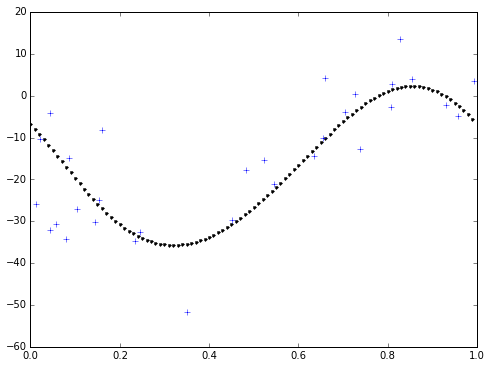
\includegraphics[width=1\textwidth, height=7.5cm]{radialvelocity.png}
\end{figure}
\end{block}
\end{textblock}

\begin{textblock}{14.00}(15.0,2)
\begin{block}{Hydrodynamics in cube}
Solution of the hydrodynamics equation in the various astrophysical configuration is one of the 
major problem in numerical astrophysics. Basic principles of the numerical hydrodynamics can 
be shown on the solution of the Burgers equation easily coded in PYTHON. 
\begin{figure}
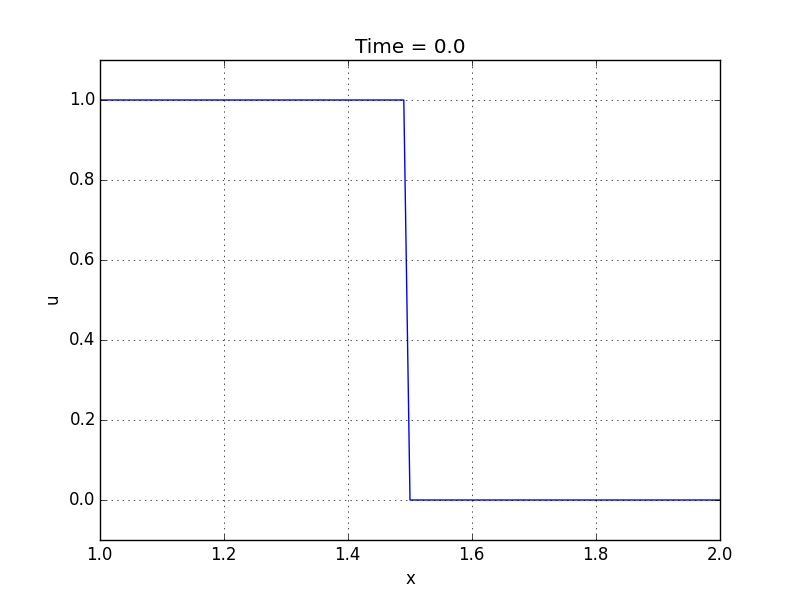
\includegraphics[width=0.5\textwidth, height=6cm]{plt1.png}
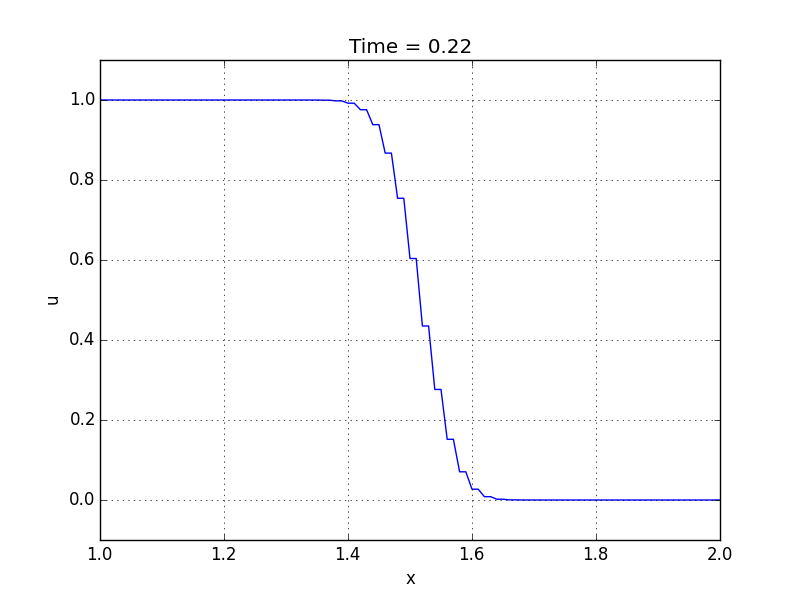
\includegraphics[width=0.5\textwidth, height=6cm]{plt2.png}\\
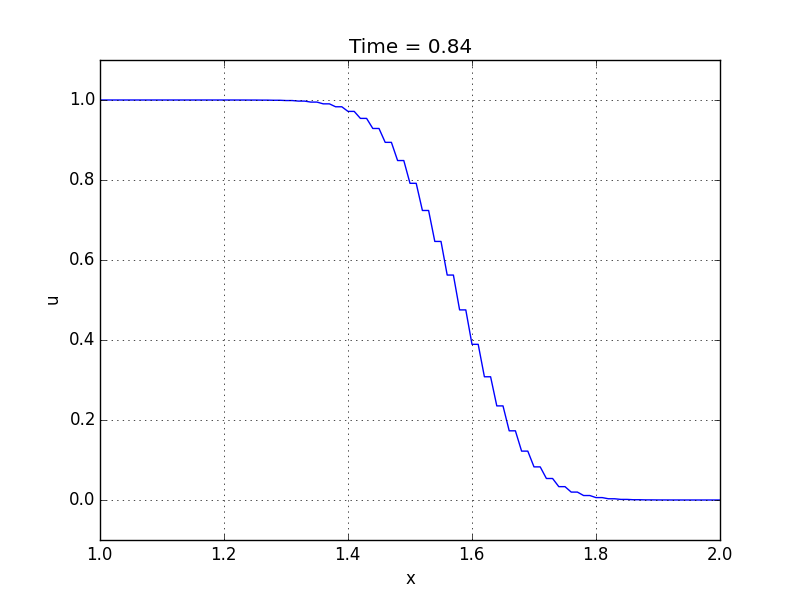
\includegraphics[width=0.5\textwidth, height=6cm]{plt3.png}
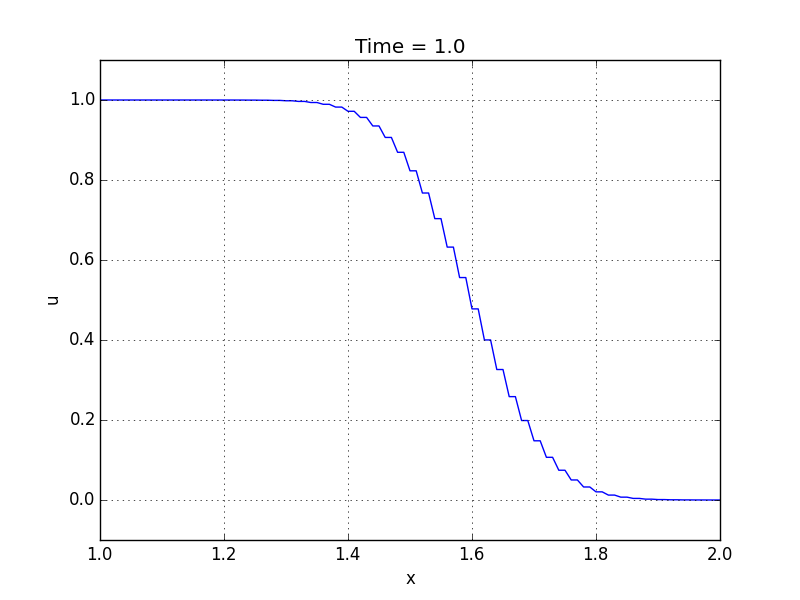
\includegraphics[width=0.5\textwidth, height=6cm]{plt4.png}\\
\end{figure}
\end{block}
\end{textblock}

\end{frame}
\end{document}

